\documentclass[12pt, a4paper]{article}
\usepackage[utf8]{inputenc}

\title{Control of robotic arm and gripper}
\author{Cristian Enrico Capalbo}
\date{\today}
\usepackage{graphicx}
\usepackage{wrapfig}
\usepackage{subcaption}
\graphicspath{ {images/} }

\begin{document}

\maketitle
\newpage
In the original design of the robot, the degrees of freedom of the arm and the gripper (the end effector) are controlled by means of a remote controller. 


\begin{figure}[ht]
	\begin{minipage}[b]{0.45\linewidth}
		\centering
		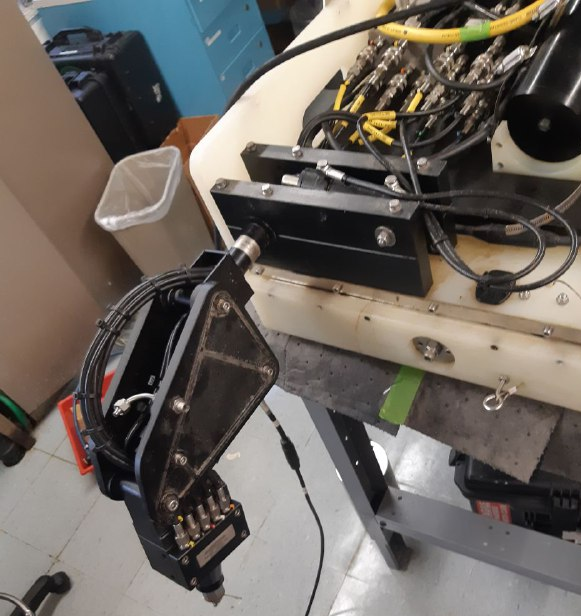
\includegraphics[width=\textwidth]{arm}
		\caption{Robotic arm}
		\label{fig:arm}
	\end{minipage}
	\hspace{0.5cm}
	\begin{minipage}[b]{0.45\linewidth}
		\centering
		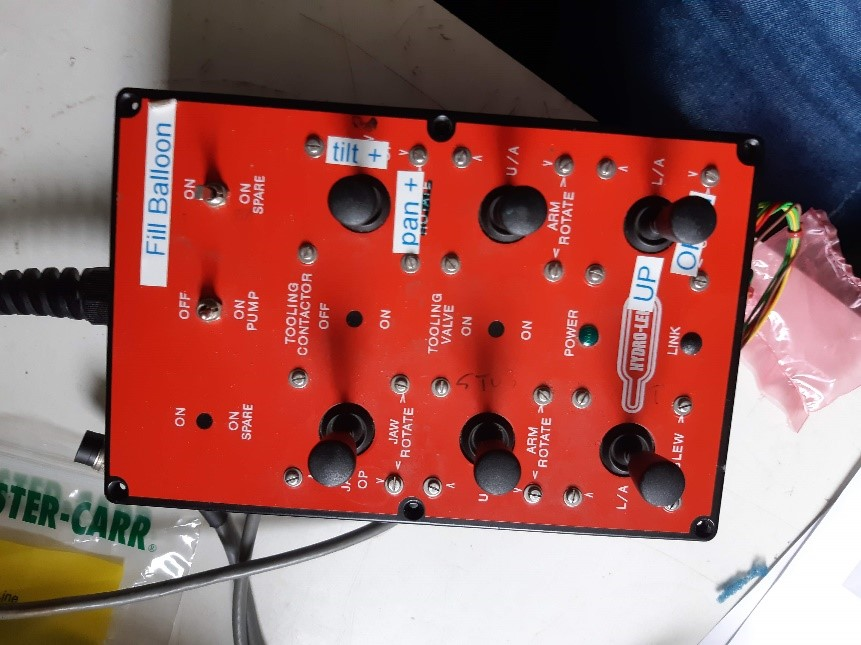
\includegraphics[width=\textwidth, angle=-90]{remote.jpg}
		\caption{Remote controller}
		\label{fig:remote}
	\end{minipage}
\end{figure}

Although this is the best solution, as it was at the start of the experience it showed a sort of a lag, since there was a delay between the moment in which the command was sent and the effective movement; also, if the command was too short the arm didn’t move at all. 
\\
At the starting point the reason of this problem was unknown, it could either be the control electronics or the hydraulic actuation of the system. We choose to examine first the electronics, then go on with the hydraulic valves if necessary.
\\ 


The electronic system consists initially of a printed board, housed in the remote, to which all the cables from the several joysticks are connected. This board reads the analogic signals and sends them to the on-board controller of the valves through an ethernet connection. The printed board contains some chips that could cause the delay, and each of them has been analysed.

\begin{figure}[h]
	
	\begin{subfigure}[t]{0.5\textwidth}
		\centering
		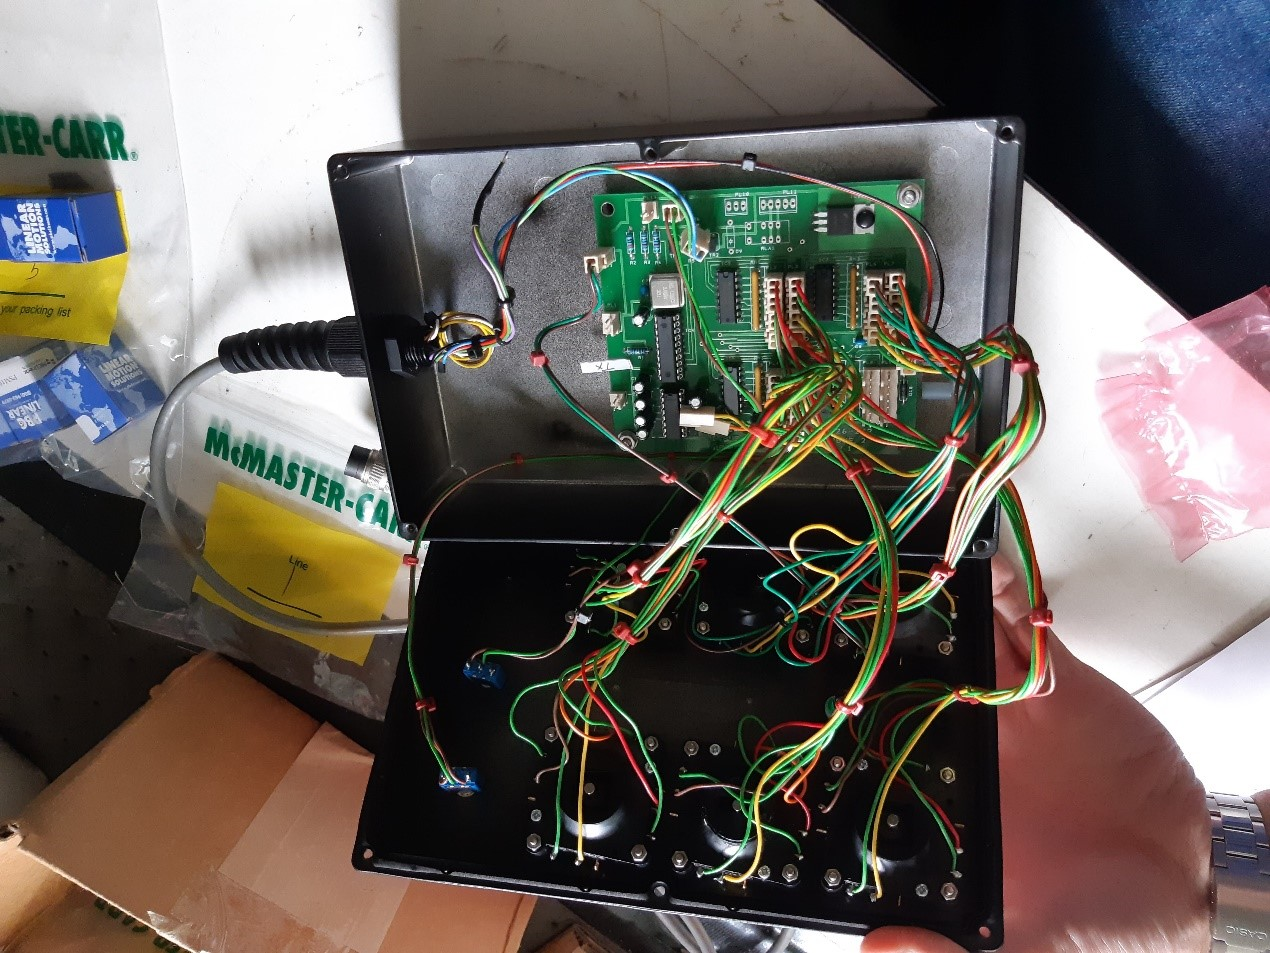
\includegraphics[width=\textwidth]{remote_internal} 
		\caption{Internal parts of the remote}
		\label{fig:remote_in}
	\end{subfigure}
	
	\begin{subfigure}[t]{0.5\textwidth}
		\centering
		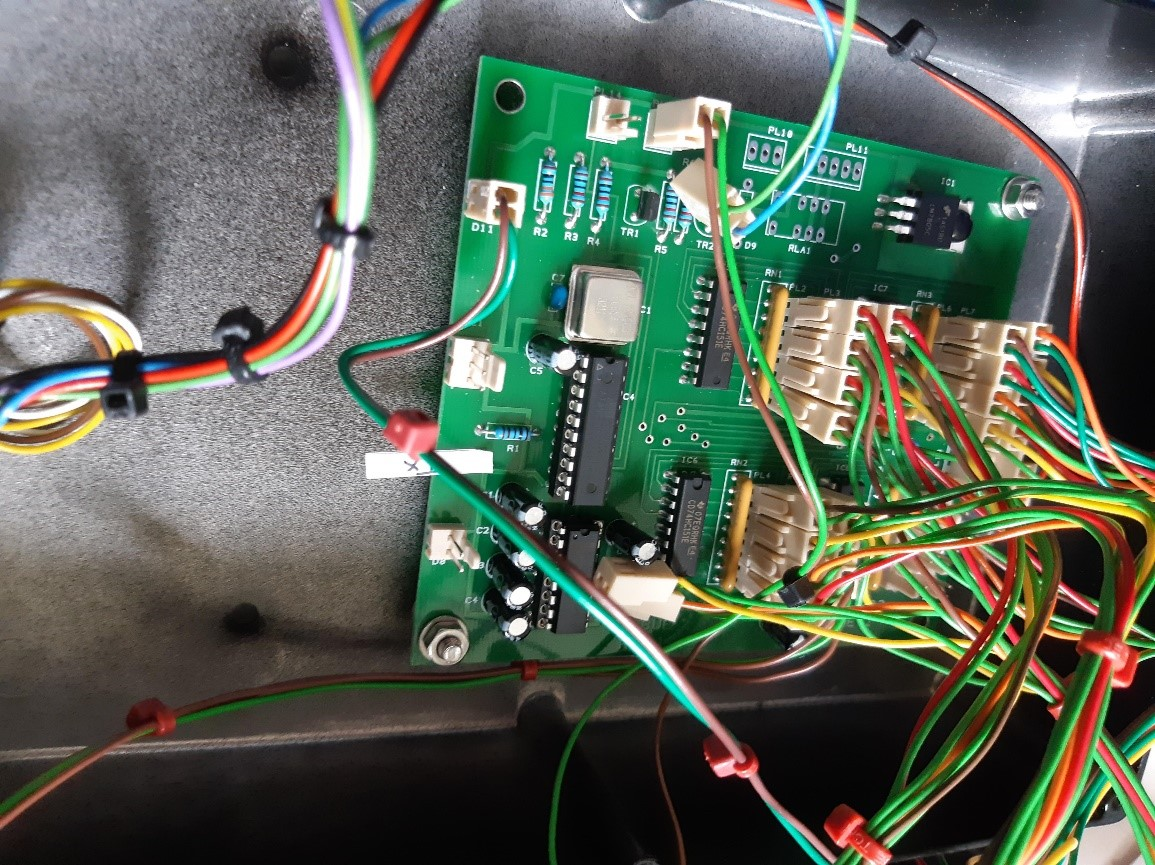
\includegraphics[width=\textwidth]{remote_board}
		\caption{Electrical board of the remote}
		\label{fig:remote_board}
	\end{subfigure}
 
	\caption{Components of the remote}
	\label{fig:remote_comp}
\end{figure}

\end{document}